\documentclass[a4paper]{article}

%use the english line for english reports
%usepackage[english]{babel}
\usepackage[portuguese]{babel}
\usepackage[utf8]{inputenc}
\usepackage{indentfirst}
\usepackage{graphicx}
\usepackage{verbatim}
\usepackage{listings}


\begin{document}

\setlength{\textwidth}{16cm}
\setlength{\textheight}{22cm}

\title{\Huge\textbf{Ni-ju}\linebreak\linebreak\linebreak
\Large\textbf{Relatório Intercalar}\linebreak\linebreak
\linebreak\linebreak

\includegraphics[scale=0.1]{../printscreens/feup-logo.png}\linebreak\linebreak
\linebreak\linebreak
\Large{Mestrado Integrado em Engenharia Informática e Computação} \linebreak\linebreak
\Large{Programação em Lógica}\linebreak
}

\author{\textbf{Grupo Niju\_2:}\\
João Pedro Furriel de Moura Pinheiro - up201104913\\
Ventura de Sousa Pereira - up201404690\\
\linebreak\linebreak \\
 \\ Faculdade de Engenharia da Universidade do Porto \\ Rua Roberto Frias, s\/n, 4200-465 Porto, Portugal \linebreak\linebreak\linebreak
\linebreak\linebreak\vspace{1cm}}

\maketitle
\thispagestyle{empty}

%************************************************************************************************
%************************************************************************************************

\newpage

%Todas as figuras devem ser referidas no texto. %\ref{fig:codigoFigura}
%
%%Exemplo de código para inserção de figuras
%%\begin{figure}[h!]
%%\begin{center}
%%escolher entre uma das seguintes três linhas:
%%\includegraphics[height=20cm,width=15cm]{path relativo da imagem}
%%\includegraphics[scale=0.5]{path relativo da imagem}
%%\includegraphics{path relativo da imagem}
%%\caption{legenda da figura}
%%\label{fig:codigoFigura}
%%\end{center}
%%\end{figure}
%
%
%\textit{Para escrever em itálico}
%\textbf{Para escrever em negrito}
%Para escrever em letra normal
%``Para escrever texto entre aspas''
%
%Para fazer parágrafo, deixar uma linha em branco.
%
%Como fazer bullet points:
%\begin{itemize}
	%\item Item1
	%\item Item2
%\end{itemize}
%
%Como enumerar itens:
%\begin{enumerate}
	%\item Item 1
	%\item Item 2
%\end{enumerate}
%
%\begin{quote}``Isto é uma citação''\end{quote}


%%%%%%%%%%%%%%%%%%%%%%%%%%
\section{O Jogo Ni-ju}

Ni-ju (20, em japonês) é um jogo desenvolvido pelo designer e artista Néstor Romeral Andrés, em 2016, tendo sido publicado pela HenMar Games, nestorgames.
O jogo é constituido por 40 peças, sendo estas divididas por cor - branca e preta, entre os jogadores, ficando, cada um, com 20 peças de padrões diferentes (daí o nome do jogo). Cada peça tem um padrão desenhado com pontos.
Cada jogador deverá colocar uma peça na zona de jogo, seguido pelo seu adversário.
Antes de jogar uma peça, o jogador pode rodar a mesma 90, 180 ou 270 graus para, desta forma, rodar o padrão que a peça representa.
O objetivo do jogo é recriar o padrão descrito na peça, à volta da mesma. No final ganha quem conseguir recriar mais padrões, quando se esgotarem as peças.
Nesta versão que desenvolveremos, o jogo termina quando todas as peças forem colocadas na mesa. Nesta versão,os discos de ajuda que são visíveis na imagem tamb´ém não serão utilizados.
\linebreak\linebreak\\
\textbf{Regras}:
  A única regra do jogo prende-se com a colocação das peças. Uma peça apenas poderá ser colocada numa posição adjacente (em cima, por baixo, à esquerda ou à direita) a outra peça que já esteja colocada na mesma.
\linebreak\linebreak\\

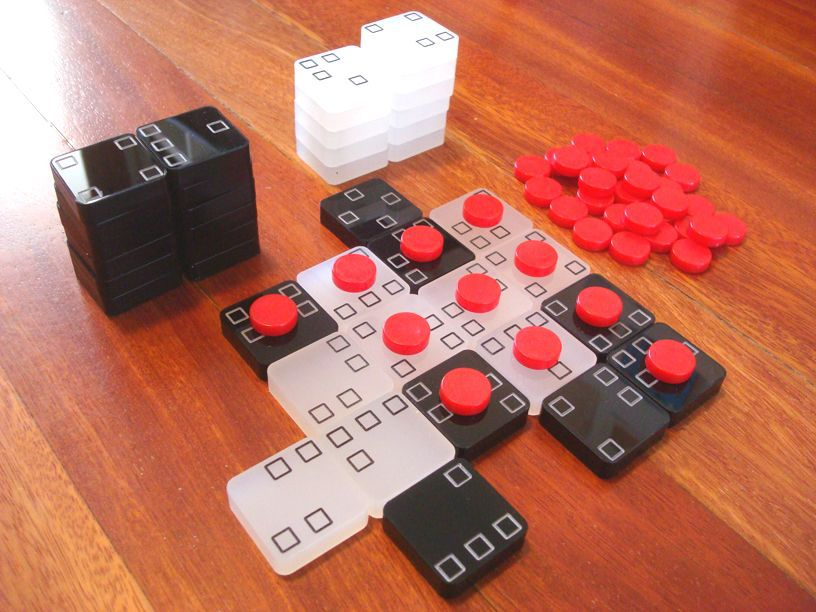
\includegraphics[scale=0.3]{../printscreens/niju.jpg} \linebreak


%%%%%%%%%%%%%%%%%%%%%%%%%%
\section{Representação do Estado do Jogo}

Inicialmente, o estado inicial do jogo será uma lista que represente um espaço vazio, visto que este é dinâmico. Modifica-se conforme a posição de cada peça jogada.

\textbf{Estado Inicial}:

[
  [
      [[-1, -1, -1],
		  [-1, -1, -1],
		  [-1, -1, -1]
		 ]
                      ]
	                 ]\linebreak\linebreak\\

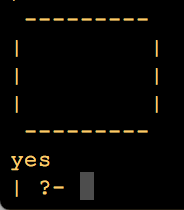
\includegraphics[scale=0.8]{../printscreens/initial_board.png} \linebreak


Num estado intermédio, o jogo terá algumas peças em jogo.

\textbf{Possível representação}:

	[
		%row1
		[

		 [[0, 1, 1],
		  [0, 0, 1],
		  [0, 0, 1]
		 ],

		 [[0, 2, 2],
		  [0, 0, 0],
		  [2, 0, 2]
		 ]

		],

		%row2

		[

		 [[-1, -1, -1],
		  [-1, -1, -1],
		  [-1, -1, -1]
		 ],

		 [[1, 0, 1],
		  [0, 0, 0],
		  [1, 0, 1]
		 ]

		]

	]\linebreak\linebreak\\

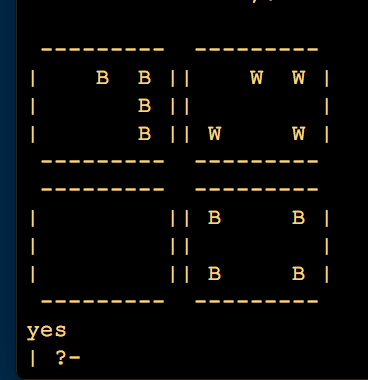
\includegraphics[scale=0.8]{../printscreens/intermediate_board.png} \linebreak

O estado final é quando todas as peças já foram colocadas. Num hipotético jogo apenas com 11 peças, este seria um possível estado final.

\textbf{Representação final}:

[

		%row1

		[

		 [[2, 0, 0],
		  [2, 0, 0],
		  [2, 0, 2]
		 ],

		 [[2, 0, 0],
		  [0, 0, 2],
		  [0, 2, 2]
		 ],

		 [[0, 2, 0],
		  [0, 0, 0],
		  [2, 2, 2]
		 ],

		 [[1, 0, 0],
		  [1, 0, 0],
		  [1, 0, 1]
		 ]

		],


		%row2

		[

		 [[-1, -1, -1],
		  [-1, -1, -1],
		  [-1, -1, -1]
		 ],

		 [[2, 2, 2],
		  [0, 0, 2],
		  [0, 0, 0]
		 ],

		 [[0, 0, 2],
		  [2, 0, 2],
		  [2, 0, 0]
		 ],

		 [[0, 0, 1],
		  [1, 0, 1],
		  [1, 0, 0]
		 ]

		],

		%row3

		[

		 [[1, 0, 0],
		  [0, 0, 1],
		  [1, 1, 0]
		 ],

		 [[1, 1, 1],
		  [0, 0, 1],
		  [0, 0, 0]
		 ],

		 [[0, 0, 2],
		  [2, 0, 2],
		  [2, 0, 0]
		 ],

		 [[0, 0, 1],
		  [1, 0, 1],
		  [1, 0, 0]
		 ]

		]

	]\linebreak\linebreak\\

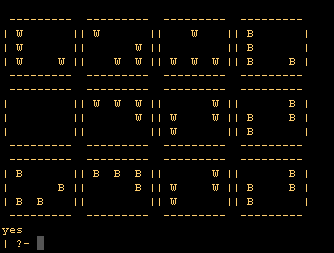
\includegraphics[scale=0.6]{../printscreens/winning_board.png} \linebreak




%%%%%%%%%%%%%%%%%%%%%%%%%%
\section{Visualização do Tabuleiro}

O padrão de cada peça é representado por B's ou W's, dependendo se a peça é preta ou branca, respetivamente. Os espaços vazios no tabuleiro são representados por uma matriz, de 3x3, de espaços. Além disso, os espaços vazios da peça são, também, representados por espaços.

\textbf{Predicados usados para a impressão do tabuleiro}:
\begin{lstlisting}
printElement(X) :- X =:= 1, write(' B ').
printElement(X) :- X =:= 2, write(' W ').
printElement(X) :- X =:= -1, write('   ').
printElement(X) :- X =:= 0, write('   ').
printPieceRowSeparation(BoardRow) :-

	BoardRow = [].

printPieceRowSeparation(BoardRow) :-

	BoardRow \= [],
	[\_ | Rest] = BoardRow,
	write(' --------- '),
	printPieceRowSeparation(Rest).

printPieceRow([X1,X2,X3]) :-

	write('|'),
	printElement(X1),
	printElement(X2),
        printElement(X3),
	write('|').


printBoard(Board) :-

	Board = [].

printBoard(Board) :-

	[Row | Rest] = Board,
	printPieceRowSeparation(Row),
	nl,
	printPiecesRow1(Row),
	nl,
	printPiecesRow2(Row),
	nl,
	printPiecesRow3(Row),
	nl,
	printPieceRowSeparation(Row),
	nl,
	printBoard(Rest).

printPiecesRow1(BoardRow) :-

	BoardRow = [].

printPiecesRow1(BoardRow) :-

	[Piece | Rest] = BoardRow,
	[PieceRow1 | \_] = Piece,
	printPieceRow(PieceRow1),
	printPiecesRow1(Rest).


printPiecesRow2(BoardRow) :-
	BoardRow = [].

printPiecesRow2(BoardRow) :-
	[Piece | Rest] = BoardRow,
	[\_,PieceRow2,\_] = Piece,
	printPieceRow(PieceRow2),
	printPiecesRow2(Rest).


printPiecesRow3(BoardRow) :-

	BoardRow = [].

printPiecesRow3(BoardRow) :-

	[Piece | Rest] = BoardRow,
	[\_,\_,PieceRow3] = Piece,
	printPieceRow(PieceRow3),
	printPiecesRow3(Rest).
\end{lstlisting}


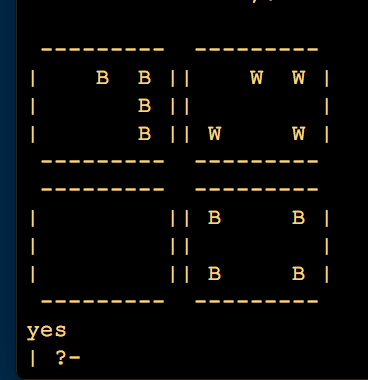
\includegraphics[scale=0.5]{../printscreens/intermediate_board.png} \linebreak

%%%%%%%%%%%%%%%%%%%%%%%%%%
\section{Movimentos}

\begin{lstlisting}
	playPieceRight(CurrentBoard, Piece, Rotation, Row, Column, ResultingBoard).
	playPieceDown(CurrentBoard, Piece, Rotation, Row, Column, ResultingBoard).
	playPieceLeft(CurrentBoard, Piece, Rotation, Row, Column, ResultingBoard).
	playPieceUp(CurrentBoard, Piece, Rotation, Row, Column, ResultingBoard).
\end{lstlisting}

Os parâmetros dos predicados das jogadas são:

\begin{lstlisting}
	CurrentBoard - Estado atual do jogo.
	Piece - A peça a ser jogada.
	Rotation - A rotação da peça (0, 90, 180 ou 270 graus).
	Row - A linha onde será colocada a peça.
	Column - A coluna onde será colocada a peça.
	ResultingBoard - O estado do jogo após a colocação da peça.
\end{lstlisting}

Antes de efectivamente colocar a peça na mesa, serão desenvolvidos predicados para a validação da jogada, isto é, para garantir que a regra da colocação da peça seja cumprida, e apenas nesse caso, a peça seja colocada na mesa.

\end{document}
